\chapter{Concetti di Base}

\section{Introduzione}

In questo corso verrà studiata l'architettura interna e il funzionamento dei processori moderni (con riferimento a cache e RAM).

\nt{Lo scopo del corso è quello di spiegare il passaggio al multi-core, subito dopo la "Rivoluzione RISC".}

\begin{figure}[h]
    \centering
    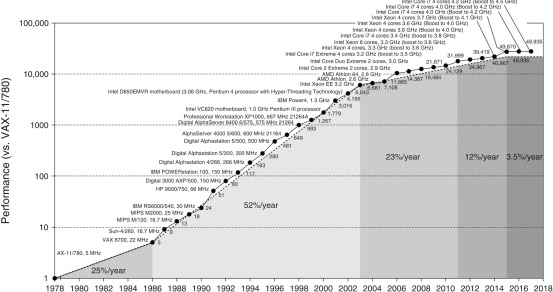
\includegraphics[scale=0.9]{01-ConcettiDiBase/Evoluzione.jpg}
    \caption{Nel 1986 ha inizio la "Rivoluzione RISC", mentre all'inizio degli anni 2000 si inizia a sfruttare l'idea di avere più "core".}
\end{figure}

\subsection{Tassonomia delle architetture}

Il contenuto del corso può essere descritto dalla "Tassonomia di Flynn". 

\dfn{Tassonomia di Flynn}{
  La Tassonomia di Flynn organizza i vari tipi di processori in base a determinate caratteristiche che verranno approfondite in questo corso.
}

\begin{figure}[h]
    \centering
    \includegraphics{01-ConcettiDiBase/TassonomiaDiFlynn.png}
    \caption{La Tassonomia di Flynn}
\end{figure}

\subsection{Alcuni concetti fondamentali}

\dfn{Microarchitettura}{
  L'architettura interna di un processore: com'è fatto a partire dal suo datapath.
}

\cor{Datapath}{
  Il percorso che compiono le istruzioni all'interno del processore per venire eseguite.
}

\nt{Diversi tipi d'istruzioni percorrono diverse parti del datapath per venire eseguite.}

\dfn{ISA}{
  L'Instruction Set Architetture (ISA) è l'insieme d'istruzioni macchina di un processore.
}

\nt{Due processori possono avere lo stesso ISA, ma microarchitetture diverse (e.g. AMD e Intel).}

\section{Una semplice macchina RISC}

\qs{}{Qual è la differenza tra un processore a 32 bit e un processore a 64 bit?}

\paragraph{Risposta:} il processore a 64 bit manipola in maniera naturale informazione scritta con 64 bit e il processore a 32 bit manipola in maniera naturale informazione scritta con 32 bit.

\subsubsection{Caratteristiche fondamentali dell'architettura RISC:}

\begin{itemize}
  \item [$\Rightarrow$] le istruzioni hanno tutte la stessa lunghezza (o a 32 bit o a 64 bit);
  \item [$\Rightarrow$] le istruzioni sono semplici;
  \item [$\Rightarrow$] la Control Unit è semplice (poche porte logiche, quindi frequenze di clock più elevate).
\end{itemize}

\nt{Ciò che verrà descritto in questa sezione è una versione semplificata di MIPS, la prima macchina RISC.

  Si considerano 32 registri a 32 bit e si ignorano le operazioni floating point.
}


\begin{figure}[h]
    \centering
    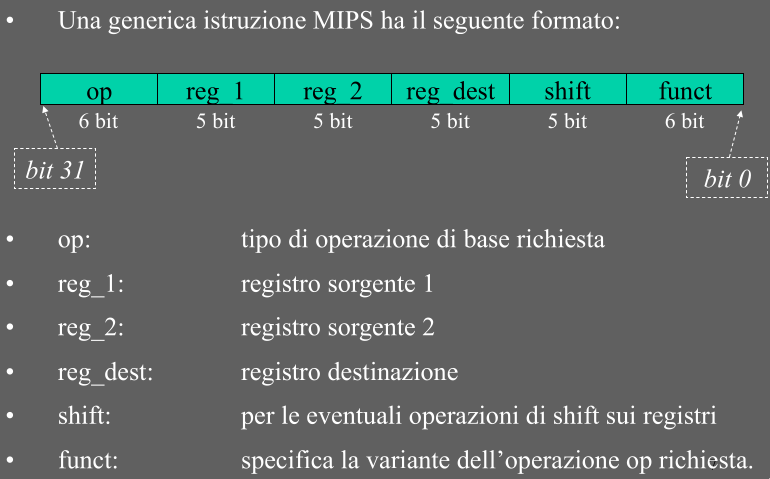
\includegraphics[scale=0.5]{01-ConcettiDiBase/MIPS.png}
    \caption{Istruzione MIPS}
\end{figure}

\dfn{Istruzioni di tipo-R}{
  Le istruzioni di tipo-R usano due registri e restituiscono il risultato a un terzo registro. La convenzione prevede che il campo OP sia 0. L'operazione specifica si trova nel campo func.
}

\nt{Solitamente si usa la lettera D quando si parla di dati interi (DADD, DSUB, etc.), F per i floating point.}

\dfn{Istruzioni di tipo-I}{
  Le istruzioni di tipo-I usano un valore immediato. La convenzione prevede che il campo op sia 8.
}

\dfn{LOAD e STORE}{
  La LOAD carica in un registro un valore che si trova in memoria (op = 35). La STORE salva in memoria il valore di un registro (op = 43).
}

\dfn{Salti condizionati (BRANCH)}{
  Salta solo se si verifica una determinata condizione (op = 5). 
}

\dfn{Salti incondizionati (JUMP)}{
  Salta sempre (op = 4). 
}

\subsection{MIPS - Versione monociclo}

Generalmente i primi due passi di ogni istruzione sono:

\begin{enumerate}
  \item Usa il Program Counter (PC) per prelevare dalla "memoria d'istruzioni\footnote{Cache di primo livello.}" la prossima istruzione da eseguire;
  \item Decodifica l'istruzione e contemporaneamente legge i registri.
\end{enumerate}

\nt{I passi successivi dipendono dal tipo d'istruzione (tutte usano la ALU).}

\begin{itemize}
  \item [$\Rightarrow$] LOAD e STORE accedono alla memoria dati e nel caso di LOAD viene aggiornato un registro;
  \item [$\Rightarrow$] le istruzioni logico-aritmetiche aggiornano un registro;
  \item [$\Rightarrow$] le istruzioni di salto possono alterare il valore di PC.
\end{itemize}

\begin{figure}[h]
    \centering
    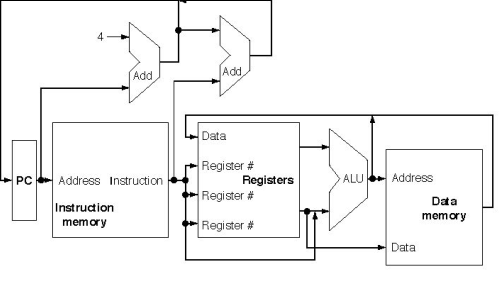
\includegraphics[scale=0.8]{01-ConcettiDiBase/MIPS2.png}
    \caption{Schema ad alto livello del datapath MIPS}
\end{figure}

\nt{Il fluire delle informazioni nel datapath deve essere controllato da una "Control Unit".}

\begin{figure}[h]
    \centering
    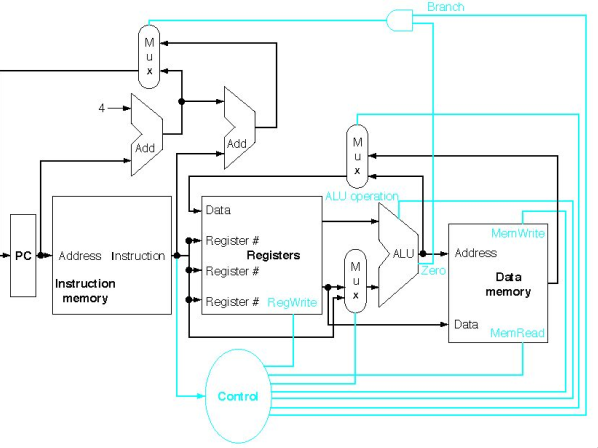
\includegraphics[scale=0.8]{01-ConcettiDiBase/MIPS3.png}
    \caption{Versione modificata del MIPS con una Control Unit}
\end{figure}

\nt{L'esecuzione di ciascuna istruzione può avvenire in un unico ciclo di clock, purché sia stato adeguatamente dimensionato.}

\subsubsection{Per capire come funziona il datapath di una macchina monociclo si osserva che esso è composto da due tipi di elementi logici:}

\begin{itemize}
  \item [$\Rightarrow$] gli elementi di \textit{stato};
  \item [$\Rightarrow$] gli elementi di tipo \textit{combinatorio}.
\end{itemize}

\dfn{Elementi di stato}{
  Gli elementi di stato sono quelli in grado di memorizzare uno \textit{stato} (e.g. flip flop, registri e memorie). Un elemento di stato possiede almeno 2 ingressi e un'uscita. Gli ingressi richiedono:
  \begin{itemize}
    \item [$\Rightarrow$] il valore da scrivere nell'elemento;
    \item [$\Rightarrow$] il clock per determinare quando scriverlo.
  \end{itemize}

  Il dato presente in uscita è sempre quello scritto in un ciclo di clock precedente.
}

\nt{Solitamente esiste un terzo ingresso "di controllo" che stabilisce se l'elemento di stato può effettivamente memorizzare l'input.}

\dfn{Elementi combinatori}{
  Gli elementi combinatori sono quelli in cui le uscite dipendono solamente dai valori d'ingresso in un dato istante (e.g. ALU e Multiplexer). 
}

\subsection{Banco dei registri}

\dfn{Banco dei registri}{
  Nelle immagini precedenti i registri della CPU sono rappresentati da un'unità funzionale detta \textit{register file} (o banco dei registri). Essa è un'unità di memoria molto piccola e veloce.
}

\nt{Si può accedere a ognuno dei 32 registri (da 0 a 31) specificando il suo indirizzo. Ogni registro può essere letto o scritto.}

\paragraph{Operazione di scrittura:} quando il segnale di controllo (RegWrite) è a 1, il valore proveniente dalla ALU o dalla Data Memory e presente in input in \textit{DST data} viene memorizzato nel registro di destinazione specificato da \textit{DST addr}.
 

\begin{figure}[h]
    \centering
    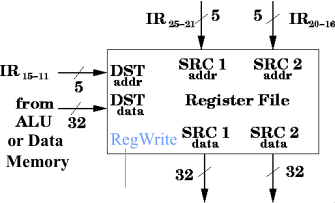
\includegraphics[scale=0.6]{01-ConcettiDiBase/scrittura.png}
    \caption{Operazione di scrittura}
\end{figure}

\paragraph{Operazione di lettura:} le letture sono immediate. In qualunque momento alle uscite \textit{SRC1 data} e \textit{SRC2 data} è presente il contenuto dei registri i cui numeri sono specificati da \textit{SRC1 addr} e \textit{SRC2 addr}.


\begin{figure}[h]
    \centering
    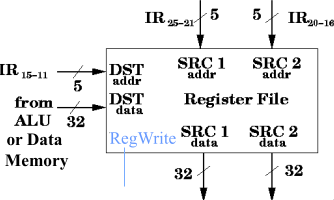
\includegraphics[scale=0.6]{01-ConcettiDiBase/lettura.png}
    \caption{Operazione di lettura}
\end{figure}

\subsection{Una semplice Control Unit}

\dfn{Control Unit}{
  La Control Unit riceve in input i 6 bit del campo op dell'istruzione e deve generare in output i segnali per comandare:

    \begin{itemize}
    \item [$\Rightarrow$] la scrittura dei registri;
    \item [$\Rightarrow$] la lettura/scrittura della memoria dati (MemRead/MemWrite);
    \item [$\Rightarrow$] i Multiplexer che selezionano gli input da usare;
    \item [$\Rightarrow$] la ALU (ALUOp) che deve eseguire ciascuna operazione aritmetico-logica appropriata per la specifica istruzione in esecuzione.
  \end{itemize}
}

\cor{Segnale ALUOp}{
  Il segnale ALUOp dipende:
  \begin{itemize}
    \item [$\Rightarrow$] dal tipo d'istruzione in esecuzione, specificato nel campo op;
    \item [$\Rightarrow$] dalla specifica operazione da eseguire, determinata dal campo func.
  \end{itemize}
}

\ex{Istruzioni di tipo-R}{
  \begin{itemize}
    \item [$\Rightarrow$] Se op == load || op == store allora la ALU deve eseguire una \textit{somma};
    \item [$\Rightarrow$] se op == beq allora la ALU deve eseguire una \textit{sottrazione} (per controllare se il risultato è 0);
    \item [$\Rightarrow$] Se op == tipo-R allora è il campo \textit{func} a stabilire l'operazione che deve eseguire la ALU.
  \end{itemize}

}

\dfn{ALU Control}{
  Parte della Control Unit che indica le operazioni da eseguire. 
}

\begin{figure}[h]
    \centering
    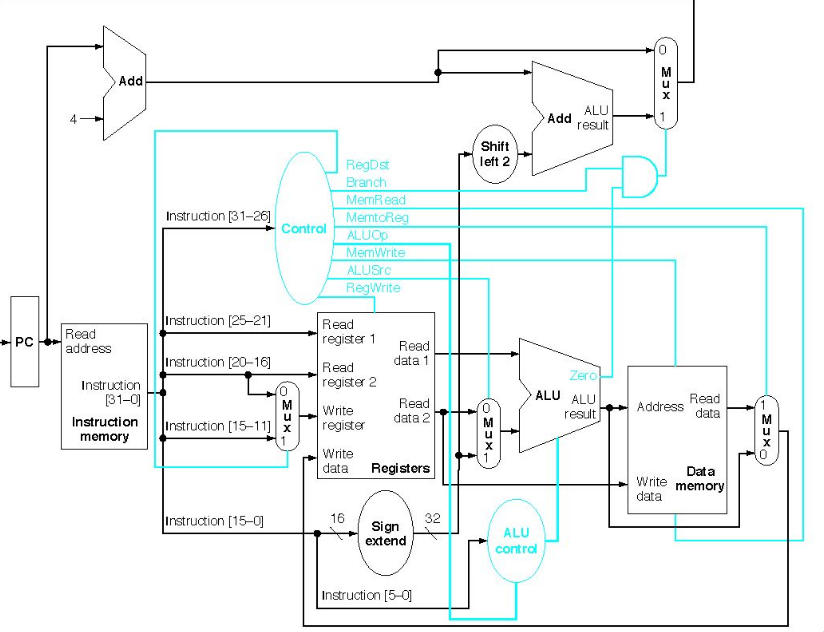
\includegraphics[scale=0.34]{01-ConcettiDiBase/MIPS4.png}
    \caption{Versione modificata del MIPS la ALU Control}
\end{figure}

\subsection{L'esecuzione di un'istruzione}

\begin{enumerate}
  \item Il contenuto del PC viene utilizzato per indirizzare la instruction memory e produrre in output l'istruzione da eseguire;
  \item Il campo \textit{op} dell’istruzione viene mandato in input alla Control
    Unit, mentre i campi \textit{reg\_1} e \textit{reg\_2} vengono usati per indirizzare il
register file;
\item La CU produce in output i nove segnali di controllo relativi a una
operazione di tipo-R, e in particolare ALUOp=10, che, dati in
input alla ALU control insieme al campo \textit{func} dell’istruzione
stabiliscono l’effettiva operazione di tipo-R che deve eseguire la
ALU;
\item Nel frattempo, il register file produce in output i valori dei due
  registri \textit{reg\_1} e \textit{reg\_2}, mentre il segnale ALUSrc=0 stabilisce che il
secondo input della ALU deve provenire dal secondo output del
register file;
\item La ALU produce in output il risultato della computazione, che
  attraverso il segnale \textit{MemtoReg} viene presentato in input al register
file (Write data).
\end{enumerate}

\nt{Tutti questi passi devono essere eseguiti nello stesso ciclo di clock.}

\section{Dal monociclo al multiciclo}

Le macchine monociclo sono estremamente inefficienti perché portano a sprecare cicli di clock nel caso di operazioni semplici. 
Per trasformare una macchina da monociclo in multiciclo si scompone l'esecuzione di ciascuna istruzione in un insieme di passi ognuno dei quali eseguibile in un singolo ciclo di clock (per cui ogni passo deve richiedere più o meno lo stesso tempo di esecuzione, perché la durata del clock va commisurata alla durata del passo più lungo). 

\nt{Le parole "passo", "fase", "stadio" e "stage" sono intercambiabili.}

\subsection{MIPS - Versione multiciclo}

\begin{figure}[h]
    \centering
    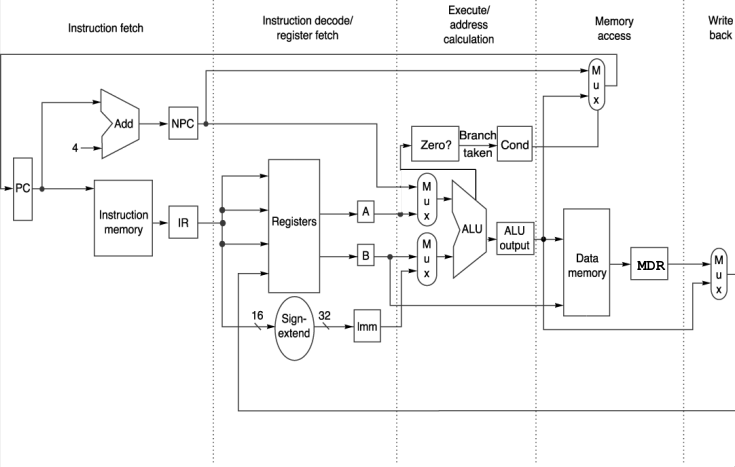
\includegraphics[scale=0.43]{01-ConcettiDiBase/MIPS5.png}
    \caption{Il Datapath suddiviso nelle 5 fasi standard}
\end{figure}

\nt{Instruction Memory e Data Memory corrispondono alla cache di primo livello (L1).}

\begin{enumerate}
  \item \textit{Instruction Fetch}: il PC indirizza le istruzioni (IR) e contemporaneamente incrementa il PC di 4 (salvato in NPC che verrà instradato alla ALU per eventuali istruzioni di salto). Da notare che la ALU non viene utilizzata quindi si potrebbe pensare di usarla al posto dell'adder, ma quando si introdurrà il concetto di \textit{pipeline} si vedrà che la ALU sarà occupata dalla fase di esecuzione di un'altra istruzione;
  \item \textit{Instruction Decode / Register Fetch}: vengono sempre prelevati i valori dei 2 registri di destinazione (anche se l'istruzione non è di tipo-R) e messi in 2 \textit{registri nascosti} A e B. Inoltre il registro Imm viene memorizzato nell'eventualità che sia un'istruzione di tipo-I. Oltre a ciò si memorizza un eventuale salto (usando un adder apposta);
  \item \textit{Execute / Address Calculation}: la ALU fa i suoi calcoli in base al tipo d'istruzione;
  \item \textit{Memory Access}: nei casi di load e store si accede alla memoria. Per la load si preleva il risultato della fase di esecuzione e viene salvato nel registro MDR. Se si sta eseguendo un'istruzione di tipo-R o di tipo-I questa fase viene saltata;
  \item \textit{Write Back:} il risultato viene scritto sul registro di destinazione. Non è necessaria per le store.
\end{enumerate}

\nt{Non necessariamente l'esecuzione di un'istruzione racchiude tutte le fasi. Ogni fase avviene in un ciclo di clock.}

\dfn{Registro "nascosto"}{
  I risultati di ciascuna fase sono memorizzati da registri "nascosti" in cui viene salvato il risultato dell'output di una fase in modo che diventi l'output della fase successiva. Non sono indirizzabili e servono solo a velocizzare l'esecuzione delle istruzioni.
}

\qs{}{Quali fasi sono coinvolte nell'esecuzione di una "load"?}

\paragraph{Risposta:} tutte.

\qs{}{Quali fasi sono coinvolte nell'esecuzione di un'istruzione di tipo-R?}

\paragraph{Risposta:} 4, perché non si deve accedere alla memoria.

\qs{}{Quali fasi sono coinvolte nell'esecuzione di una "store"?}

\paragraph{Risposta:} 4, perché non esiste la frase di Write Back.

\qs{}{Quali fasi sono coinvolte nell'esecuzione di un'istruzione di salto?}

\paragraph{Risposta:} 3, Instruction Fetch, Instruction Decode e Address Calculation.

\nt{Tutto questo è più efficiente della versione monociclo perché ogni fase usa circa $\frac{1}{5}$ del ciclo di clock e non sempre si devono attraversare tutte le fasi.}

\subsection{Control Unit multiciclo}

\dfn{Control Unit - multiciclo}{
  Ogni fase sarà descritta da una tabella di verità i cui input sono:
      \begin{itemize}
    \item [$\Rightarrow$] il tipo d'istruzione in esecuzione;
    \item [$\Rightarrow$] la fase corrente nella sequenza di esecuzione dell'istruzione.
  \end{itemize}

  L'output invece sarà:
      \begin{itemize}
    \item [$\Rightarrow$] l'insieme di segnali da asserire in quella fase;
    \item [$\Rightarrow$] la fase successiva nella sequenza di esecuzione dell'esecuzione.
  \end{itemize}

}

\nt{
  Gli output della Control Unit sono una descrizione informale di una macchina di Moore.
}

\cor{Macchina di Moore}{
  La macchina di Moore è un automa a stati finiti in cui: 
      \begin{itemize}
    \item [$\Rightarrow$] a ogni stato è associato un output che dipende solo da quello stato (i segnali da asserire);
    \item [$\Rightarrow$] la transizione nello stato successivo dipende solo dallo stato corrente e dall'input.
  \end{itemize}

}

\begin{figure}[h]
    \centering
    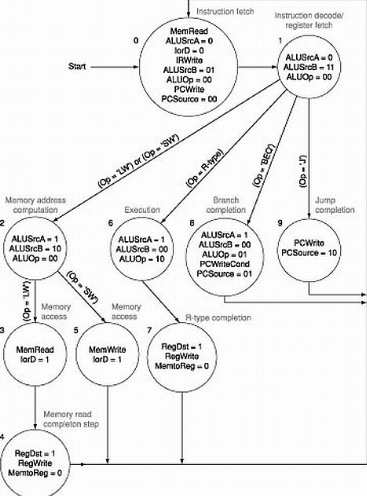
\includegraphics[scale=0.7]{01-ConcettiDiBase/CU.png}
    \caption{Unità di Controllo multiciclo}
\end{figure}

\subsection{Macchine a stati finiti e Microprogrammi}

\qs{}{Che differenza c'è tra un datapath controllato da un DFA e uno controllato da un Microprogramma?}

\paragraph{Risposta:} nessuna, è solo un modo di descrivere l'informazione. 

\dfn{Microprogrammazione}{
  Tecnica per descrivere il funzionamento della Control Unit mediante una rappresentazione simbolica del controllo in forma di microistruzioni indirizzate da un micro Program Counter.
}

\nt{Un microprogramma è solamente una rappresentazione testuale di una macchina di Moore, ogni microistruzione corrisponde a uno stato e il micro PC rappresenta il registro degli stati.}

\qs{}{Perché usare una rappresentazione o un'altra?}

\paragraph{Risposta:} è una questione di convenienza in base alla complessità della funzione (dipende sia dalle istruzioni
ISA che dalla loro scomposizione).

\nt{Per motivi storici le prime Control Unit furono descritte tramite microprogrammazione.}

\subsection{Complex Instruction Set Computer (CISC)}

Negli anni '60 e '70 l'instruction set diventa molto grande e, a posteriori, sarà chiamato CISC. In alcuni casi si raggiungevano centinaia d'istruzioni.

\dfn{Completa ortogonalità}{
  Ogni argomento di ogni istruzione poteva indirizzare la memoria usando una qualsiasi modalità d'indirizzamento possibile\footnote{Visto in "Storia dell'informatica".}.
}

\nt{Questa caratteristica permetteva molta flessibilità, ma al tempo stesso rendeva la Control Unit complicata e molto lenta.}

\qs{}{Perché si utilizzava un ISA così complesso?}

\begin{enumerate}
  \item All'epoca l'accesso alla RAM erano molto più elevati di quelli dell'accesso alla ROM che conteneva i microprogrammi per le istruzioni;
  \item Non esistevano CPU dotate di cache (introdotte solo nel 1968 e divennero di uso comune solo dopo molti anni); 
  \item Per semplificare il lavoro del programmatore;
  \item La RAM era poca e costosa, istruzioni più espressive generano eseguibili più corti;
  \item I microprogramma permettevano di aggiungere istruzioni all'instruction set.
\end{enumerate}

\subsection{Reduced Instruction Set Computer (RISC)}

Tra la fine degli anni '70 e l'inizio degli anni 80' la concezione delle architetture inizia a mutare. Nel 1980, D. Patterson e C. Sequin progettano una CPU la cui Control Unit non è descritta da un microprogramma e coniano i termini CISC e RISC.
Il loro progetto si evolverà nelle architetture SPARC (Scalable Processor ARChitecture), usate dalla SUN Microsystem. 

Contemporaneamente, J. Hennessy lavora a un'architettura simile per ottimizzare il \textit{pipeline}: MIPS (Microprocessor \textit{without} Interlocked Pipelines Stages), visto precedentemente. 

\begin{figure}[h]
    \centering
    
\includegraphics[scale=0.2]{01-ConcettiDiBase/pipeline.jpg}
    \caption{The virgin CISC vs. The chad RISC}
\end{figure}

\qs{}{Qual è l'idea alla base delle architetture RISC?}

\begin{enumerate}
  \item La CPU esegue un numero limitato d'istruzioni macchina semplici (che richiedono datapath più corti e una Control Unit semplice) e quindi avere un ciclo di clock più corto;
  \item L'accesso alla RAM va limitato il più possibile;
  \item Le istruzioni devono principalmente usare registri come argomenti.
\end{enumerate}

\subsubsection{In dettaglio:}

\begin{itemize}
  \item [$\Rightarrow$] Rinunciare a un sofisticato livello di microcodice;
  \item [$\Rightarrow$] Definire istruzioni di lunghezza fissa e facili da decodificare;
  \item [$\Rightarrow$] La memoria RAM deve essere indirizzata solo da operazioni di LOAD e STORE;
  \item [$\Rightarrow$] Avere molti registri;
  \item [$\Rightarrow$] Sfruttare la pipeline.
\end{itemize}

\nt{Questo contribuì al successo dei processori RISC che porto alla scomparsa dei CISC.}

\dfn{CPI}{
  Il Clock cycles Per Instruction (CPI) è il numero di cicli di clock necessari per eseguire un'istruzione. Indica la velocità alla quale una CPU è in grado di sfornare le istruzioni che esegue. 
}

\section{Pipeline}

\subsection{L'Architettura MIPS Pipelined}

Passando da monociclo a multiciclo si può aumentare l'efficienza, riducendo lo spreco di tempo. Ma c'è un'altra ragione: si può pensare di sovrapporre, parzialmente, istruzioni consecutive. Ciò non sarebbe possibile in una macchina monociclo. 

In una macchina multiciclo mentre una certa fase di un'istruzione occupa una certa parte del datapath le altre porzioni di datapath sono libere. 


\begin{figure}[h]
    \centering
    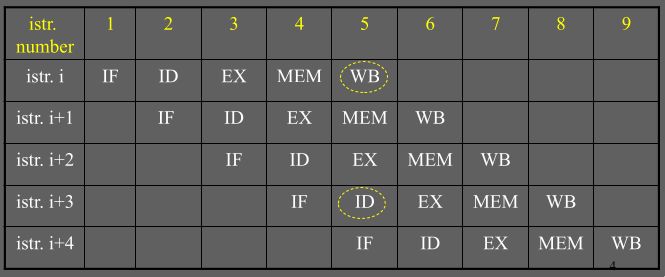
\includegraphics[scale=0.6]{01-ConcettiDiBase/pip.png}
    \caption{Rappresentazione di una pipeline.}
\end{figure}

\nt{A regime tutte le fasi sono occupate da un'istruzione diversa.}

\clm{Accorgimenti}{}{
  \begin{itemize}
    \item Si deve evitare di usare le stesse risorse per compiere contemporaneamente operazioni diverse. Per questo motivo spesso si usano più ALU;
    \item Questo è ancora più importante se si introduce il multiple issue, ossia la possibilità di eseguire istruzioni indipendenti di uno stesso programma;
    \item In alcuni casi ciò è possibile. Per esempio il banco dei registri può essere usato 2 volte in un ciclo di clock in fasi differenti (nell'immagine sopra cerchiate in giallo), uno nella prima parte del ciclo di clock e l'altro nella seconda.
  \end{itemize}
}

\begin{figure}[h]
    \centering
    
\includegraphics[scale=0.6]{01-ConcettiDiBase/pip2.png}
    \caption{Utilizzo del banco dei registri.}
\end{figure}
\pagebreak
\begin{figure}[h]
    \centering
    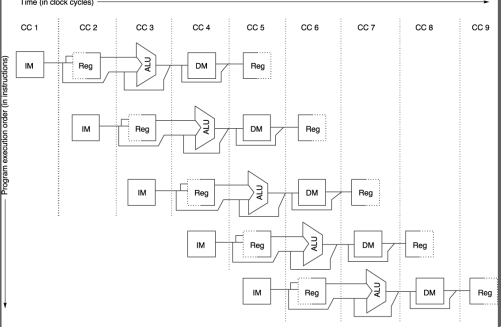
\includegraphics[scale=0.6]{01-ConcettiDiBase/mipspip.png}
    \caption{MIPS come serie di datapath traslati nel tempo.}
\end{figure}

\paragraph{Vedendo questo schema si possono fare due osservazioni:}

\begin{itemize}
  \item Si deve ipotizzare l'esistenza di memorie (cache) diverse per dati (DM) e istruzioni (IM) in modo da non avere conflitti tra IF e MEM;
  \item Il PC deve essere incrementato a ogni ciclo di clock nella fase IF.
\end{itemize}

\dfn{Registri della Pipeline}{
  In un'implementazione reale ogni stage della pipeline è separato e collegato allo stage successivo da opportuni registri della pipeline\footnote{Un po' come una catena di montaggio.}. Alla fine di un ciclo di clock il risultato viene memorizzato in uno di questi registri. 
}

\nt{Questi registri servono anche a trasportare dati d'istruzioni non adiacenti.}

\begin{figure}[h]
    \centering
    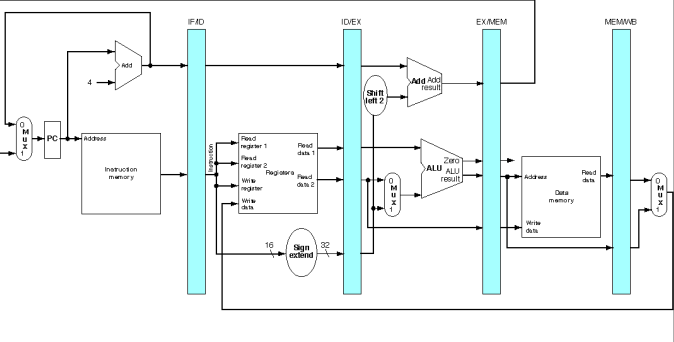
\includegraphics[scale=0.57]{01-ConcettiDiBase/regpip.png}
    \caption{Registri della pipeline (in azzurro).}
\end{figure}

\subsubsection{Simulazione di una LOAD}

\begin{itemize}
  \item \textbf{Instruction Fetch:} l'istruzione viene letta dalla Instruction Memory indirizzata dal PC e viene posta nel registro IF/ID. Il PC viene incrementato di 4 e salvato in IF/ID;
    \begin{figure}[h]
    \centering
    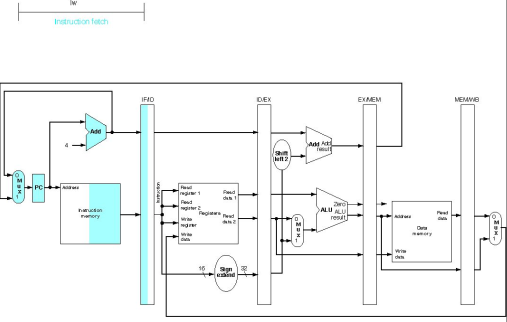
\includegraphics[scale=0.6]{01-ConcettiDiBase/L1.png}
    \caption{IF.}
\end{figure}
  \item \textbf{Instruction Decode:} il registro IF/ID viene letto per indirizzare il register file. Vengono letti i due registri, indipendentemente dal fatto che se ne userà uno solo oppure entrambi. I 16 bit del valore immediato vengono convertiti a valore 32 bit, e i 3 valori vengono scritti in ID/EX insieme al valore incrementato del PC;
    \begin{figure}[h]
    \centering
    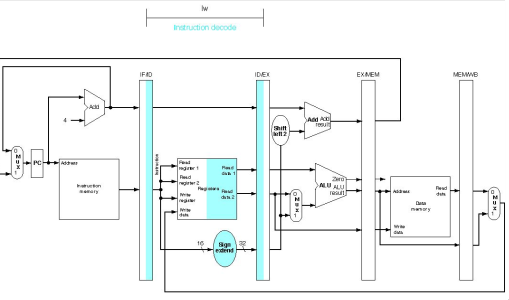
\includegraphics[scale=0.6]{01-ConcettiDiBase/L2.png}
    \caption{ID.}
\end{figure}
\pagebreak
\item \textbf{EXecute:} la load legge da ID/EX il contenuto del registro 1 e il valore immediato, li somma attraverso la ALU e scrive il risultato in EX/MEM;
    \begin{figure}[h]
    \centering
    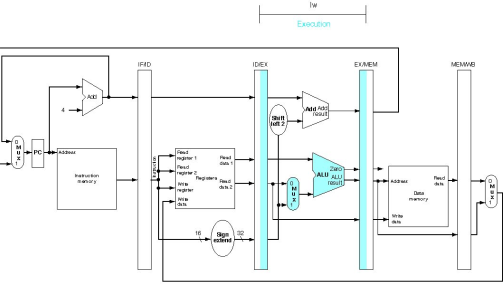
\includegraphics[scale=0.47]{01-ConcettiDiBase/L3.png}
    \caption{EX.}
\end{figure}
  \item \textbf{MEMory:} avviene l'accesso alla memoria dati, indirizzata dal valore letto nel registro EX/MEM. Il dato letto viene scritto in MEM/WB;
    \begin{figure}[h]
    \centering
    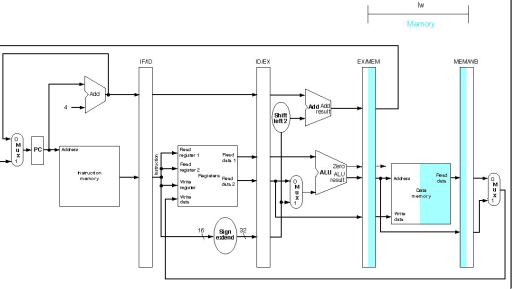
\includegraphics[scale=0.47]{01-ConcettiDiBase/L4.png}
    \caption{MEM.}
\end{figure}
  \item \textbf{Write Back:} viene scritto il registro di destinazione della load con il valore prelevato dalla memoria dati.
    \begin{figure}[h]
    \centering
    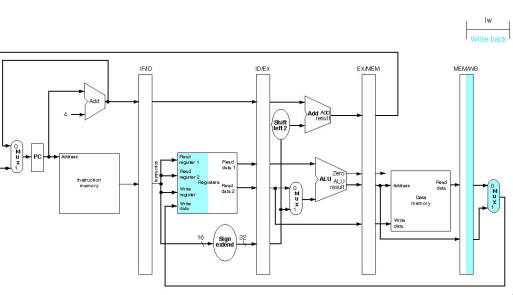
\includegraphics[scale=0.47]{01-ConcettiDiBase/L5.png}
    \caption{WB.}
\end{figure}

\end{itemize}
\pagebreak
\qs{}{Dov'è il numero del registro da modificare?}

\paragraph{Risposta:} è andato perso (sovrascritto). Per evitare ciò bisogna far sì che il numero passi attraverso tutti i registri della pipeline fino a WB.

\begin{figure}[h]
    \centering
    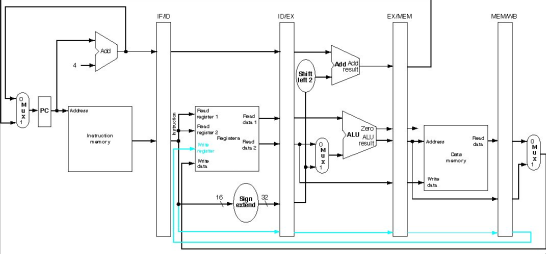
\includegraphics[scale=0.6]{01-ConcettiDiBase/New datapath.png}
    \caption{Datapath corretto.}
\end{figure}

\nt{La presenza di una pipeline rende l'esecuzione di un'istruzione leggermente più lenta di una versione senza, ma i programmi girano più velocemente.}

\subsection{Problemi della Pipeline}

Purtroppo la pipeline presenta alcuni problemi che ne limitano la produttività:

\begin{itemize}
  \item \textbf{Problemi Strutturali:} alcune combinazioni d'istruzioni non possono essere eseguite simultaneamente (e.g. se si ha una sola ALU non la si può usare nello stesso ciclo di clock per fare più cose diverse);
  \item \textbf{Problemi sui Dati:} se un'istruzione A ha bisogno del risultato di un'istruzione B precedente che non ha ancora terminato;
  \item \textbf{Problemi di Controllo:} quando vengono eseguiti salti che possono cambiare il valore di PC.
\end{itemize}

\dfn{Stall}{
  Se si verifica uno di questi problemi è necessario fermare la pipeline (stall). Se un'istruzione generica I genera un problema:
  \begin{itemize}
    \item le istruzioni avviate prima dell'istruzione I possono proseguire fino a essere completate;
    \item le istruzioni avviate dopo I devono essere fermate, fino a che non viene risolto il problema dell'istruzione I.
  \end{itemize}
}


\subsubsection{Problemi Strutturali}

\dfn{Problemi Strutturali}{
  In generale i problemi strutturali si verificano perché, per ragioni di complessità o di costi di produzione, alcune risorse hardware all'interno del datapath non sono duplicate.
}

\nt{Una cache L1 unica per dati e istruzioni genererebbe molti problemi strutturali, per questo solitamente ve ne sono 2 separate.}

\subsubsection{Problemi sui Dati}

\dfn{Problemi sui Dati}{
  I problemi sui dati sono causati dal fatto che le istruzioni di un programma non sono scollegate tra di loro e alcune devono usare output generati da istruzioni precedenti.
}

\cor{Forwarding}{
  Il forwarding è una tecnica per bypassare questi problemi. L'idea è quella di rendere disponibile un risultato il prima possibile, per esempio in una ADD il valore di output è generato prima della fase di WB. Quindi si può usare il valore memorizzato in EX/MEM dell'istruzione interessata.
}


\begin{figure}[h]
    \centering
    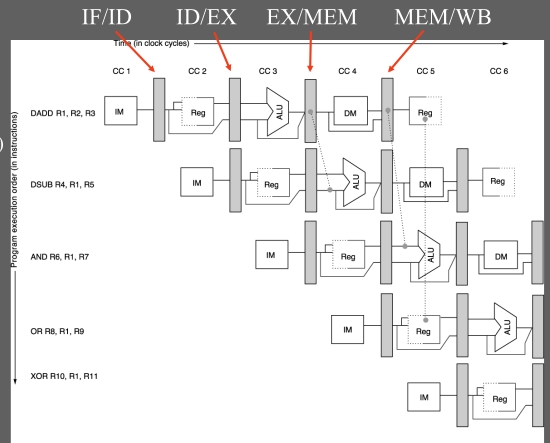
\includegraphics[scale=0.6]{01-ConcettiDiBase/Forw.png}
    \caption{Forwarding.}
\end{figure}

\subsubsection{Problemi di Controllo}

\dfn{Problemi di Controllo}{
  I problemi di controllo sono dovuti al fatto che, nel caso d'istruzioni di salto, il PC può cambiare. 
}

\nt{Si sprecano cicli di clock quando si salta. Per mitigare questo problema si usa una predizione statica: si dà per scontato che i salti in indietro vengano sempre presi e i salti in avanti no.}

\cor{Delayed Branch}{
  Il Delayed Branch consiste nello spostare dopo un branch una istruzione I che è comunque necessario eseguire indipendentemente dall'esito. In questo modo si dà tempo al datapath di valutare se il salto debba essere eseguito o meno.
}

\nt{Questa tecnica richiede l'intervento del compilatore e la CPU deve essere progettata apposta.}

\begin{figure}[h]
    \centering
    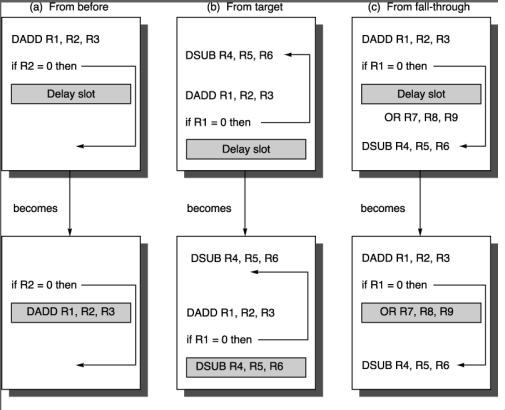
\includegraphics[scale=0.6]{01-ConcettiDiBase/Delayed.png}
    \caption{Delayed Branch.}
\end{figure}

\subsection{Multiple Pipeline}

\qs{}{Se una pipeline è efficiente, perché non usarne 2?} 

\paragraph{Bisogna che:} 

\begin{itemize}
  \item Si riescano a prelevare due istruzioni dalla instruction memory.
  \item Le due istruzioni non generino conflitti. 
  \item Le due istruzioni sono indipendenti.
\end{itemize}


Un'architettura a due pipeline era adottata dal primo pentium (80586). Una pipeline $u$ poteva eseguire qualsiasi istruzione macchina, mentre la pipeline $v$ solo istruzioni intere. 

Le istruzioni venivano eseguite \fancyglitter{in-order}, ossia nell'ordine in cui comparivano nell'eseguibile e alcune regole stabilivano se erano compatibili. Esistevano specifici compilatori per il pentium in grado di generare codice con un alto numero di istruzioni compatibili. 


\nt{Ovviamente è possibile avere più di due pipeline in parallelo.}

\paragraph{Tuttavia alcune fasi di execute sono molto lunghe rispetto alla semplice addizione tra interi:} 

\begin{itemize}
  \item Somma/sottrazione di numeri floating point. 
  \item Moltiplicazione/divisione tra numeri interi. 
  \item Moltiplicazione/divisione tra numeri floating point.
\end{itemize}

\nt{Si potrebbe adottare un ciclo di clock sufficentemente lungo per le operazioni più lente, ma ciò penalizzerebbe le operazrazioni più veloci. Conviene suddividere la execute in più fasi.} 


\begin{figure}[h]
    \centering
    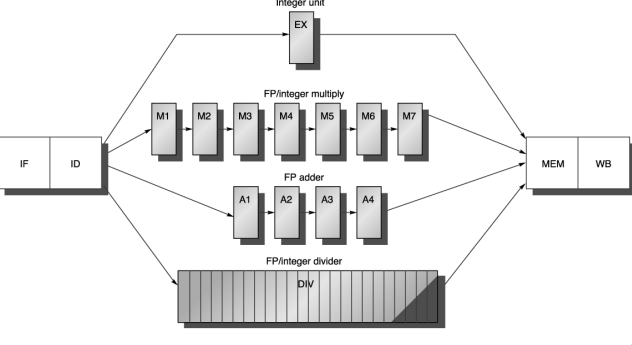
\includegraphics[scale=0.6]{01-ConcettiDiBase/pipf.png}
    \caption{Pipeline con più unità fufunzionali.}
\end{figure}

\paragraph{ In questo schema si vede:} 

\begin{enumerate}
  \item Il numero di stage della pipeline dipende dalla complessità dell'operazione. 
  \item Ci possono essere più istruzioni in fase di execute contemporaneamente.
\end{enumerate}

\subsection{Scheduling della Pipeline}

Fin'ora si è sempre assunta l'esecuzione delle istruzioni in-order, però se si verifica un problema strutturale o sui dati la pipeline viene temporaneamente fermata. Questo tipo di pipeline è detto \fancyglitter{schedulata staticamente}. 

Le CPU moderne implementano una qualche forma di \fancyglitter{scheduling dinamico}, per limitare gli stall sulla pipeline.

\dfn{IPC}{\newfancyglitter{Instruction Per Clock (cycle)}: il numero medio di istruzioni eseguite per ciclo di clock.} 

\nt{Si calcola facendo girare un benchmark di N istruzioni in C cicli di clock. 

$$IPC = N/C$$
}

\dfn{CPI}{\newfancyglitter{Clock Per Instruction} ossia il numero medio di cicli di clock necessari per eseguire un'istruzione. 
$$CPI = 1 /IPC$$
}





